\chapter{Проектирование системы формирования CAPAs на основе изменений репозитория кода} \label{ch2}

\section{Требования к системе} \label{ch2:method_selection}

Исходя из информации, полученной при анализе информационных источников были установлены следующие требования к разрабатываемой системе:

\begin{itemize}
	\item Система должна автоматически извлекать историю коммитов и связанные метрики из репозиториев GitHub (авторы, даты, количество добавленных/удалённых строк, изменения в файлах).
	\item Необходимо выполнять статический анализ кода на разных языках (например, Python, JavaScript, Java). Система должна запускать такие инструменты, как pylint, bandit для Python, eslint для JavaScript, checkstyle для Java, чтобы определить проблемы качества и уязвимости. Результаты анализа (количество предупреждений, метрики сложности и т.п.) обогащают данные коммитов.
	\item  На основании извлечённых признаков система должна определять «аномальные» изменения (например, дефектно-опасные коммиты). Здесь применяются методы Just-In-Time предсказания дефектов: обучение моделей машинного обучения для классификации коммита по риску [\ref{Hericko}].
	\item На основе обнаруженных аномалий система формирует корректирующие и предупреждающие действия. Это могут быть комментарии или автоматически созданные задачи/PR в GitHub с рекомендациями по улучшению процесса (например, «увеличить покрытие тестами», «провести рефакторинг сложного модуля»). Функционал сходен с подходом TOM: бот анализирует метрики и создает issue с описанием аномалий и действий [\ref{Bugayenko2022}].
	\item Система должна представлять результаты анализа в наглядном виде. Планируется интерактивный дашборд с графиками активности коммитов, распределением метрик и отмеченными аномальными событиями. Пользователь сможет просматривать тренды изменений и статусы CAPA.
\end{itemize}

\section{Нефункциональные требования} \label{ch2:problem_formulation}

\begin{itemize}
	\item Масштабируемость: решение должно уметь обрабатывать большие репозитории (сотни коммитов) и несколько проектов параллельно. Архитектура должна легко адаптироваться к новым языкам и инструментам. Развитием этой идеи будет наличие в проекте класса RepoAnalyzer, который будет построен универсально: для каждого типа файла в репозитории будет отображение на список анализаторов (например, {'.py': [PylintAnalyzer, BanditAnalyzer], '.js': [ESLintAnalyzer], '.java': [CheckstyleAnalyzer]}). Добавление нового языка сводится к добавлению пары (расширение → анализатор) в конфигурацию. Таким образом поддерживается гибкость и масштабируемость системы.
	\item  Отказоустойчивость: система должна корректно обрабатывать неуспешные запросы к API (повторять/логировать ошибки) и обеспечивать целостность данных.
	\item Интерпретируемость: интерфейс (дашборд) должен быть интуитивно понятным для пользователя и информативным. Информация на графиках должна быть исчерпывающей для понимания процесса разработки. Предложенные CAPA должны чётко определять найденную проблему.
	\item Безопасность: для взаимодействия с GitHub используются официальные API и безопасное храненилище токенов. 
	\item Интеграция: Механизм выдачи CAPA для разработчиков оформляется в виде GitHub-Pull Request, что упростит интеграцию с процессом разработки.
\end{itemize}

\section{Выбор технологий и инструментов} \label{ch2:algorithm_selection}

Основным языком разработки был выбран Python. Благодаря богатой экосистеме библиотек для анализа данных и машинного обучения. В частности, pandas обеспечивает удобную обработку табличных данных, scikit-learn – основа для обучение моделей классификации. Альтернативы (например, C++ или Java) имеют аналогичные библиотеки, но Python позволяет быстро прототипировать и интегрировать различные компоненты (API, ML, веб).

Для доступа к данным репозиториев (коммиты, файлы, статистика изменений). Используется GitHub API. Альтернатива – локальное клонирование через git CLI, но API быстрее предоставляет аггрегированные данные (например, статистику добавлений/удалений).

Dash + Plotly: Выбран для разработки веб-интерфейса/дашборда. Dash – высокоуровневый фреймворк на Python, построенный поверх Flask и React, облегчает создание интерактивных приложений с помощью Python-кода. Dash даёт большую гибкость в настройке интерфейса и графиков. Plotly обеспечивает красивые и интерактивные графики без необходимости писать JavaScript.

pandas: Де-факто стандарт для работы с данными в Python. Позволяет быстро агрегировать и трансформировать данные коммитов перед подачей в модели. Альтернативы: использовать NumPy напрямую или базы данных, но pandas удобнее для аналитики и визуализации.

KMeans: Используется для кластеризации коммитов и определения «границы аномалии». Алгоритм прост и хорошо масштабируется. Идея – отсортировать коммиты по удалённости до центра кластера и пометить самые далекие как аномалии. Альтернативы могли быть методы на основе плотности (DBSCAN) или статистического анализа, но KMeans достаточно для первоначального порога, при этом не требуется ввод дополнительных сложных гиперпараметров.

Статические анализаторы: Pylint (строгий линтер для Python), Bandit (фокус на уязвимости Python), ESLint (статический анализ JS/TS), Checkstyle (Java). Эти инструменты бесплатны, широко используются в индустрии и генерируют стандартизованный вывод, удобный для парсинга. Например, альтернативный SonarQube/CodeQL требовал бы более тяжёлой инфраструктуры, тогда как легковесные линтеры легко интегрировать в пайплайн. Выбор pylint/ESLint обусловлен их широкой поддержкой сообществом и гибкостью настроек.

\section{Архитектура системы} \label{ch2:2.4}

Проектируемая система реализована с учётом модульного, расширяемого и масштабируемого подхода. Архитектура разделена на несколько ключевых компонентов, которые взаимодействуют последовательно, обеспечивая надёжный сбор, обработку, анализ и визуализацию данных из репозиториев GitHub. Проектируемая система имеет модульную архитектуру с элементами сервисно-ориентированного подхода и частично реализует клиент-серверную модель.

\begin{figure}[ht]
	\centering
	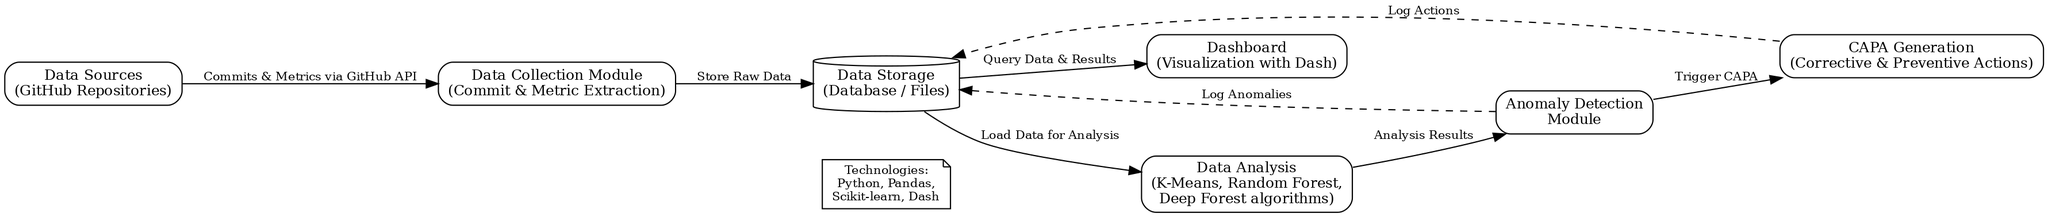
\includegraphics[width=0.8\textwidth]{my_folder/images/architect.png}
	\caption{Архитектура системы анализа коммитов и формирования CAPA}
	\label{fig:architecture_diagram}
\end{figure}

Основная идея архитектуры — разделение задач по функциональным блокам, что обеспечивает:

\begin{itemize}
	\item Модульность: каждый компонент реализует отдельную функцию, позволяя изменять или улучшать его независимо от остальных;
	\item Расширяемость: легко добавлять новые анализаторы, модели или визуализации без глобальных изменений;
	\item Производительность: локальное хранение и анализ кода минимизируют избыточные обращения к API GitHub и снижают задержки;
	\item Отказоустойчивость: чёткая обработка ошибок и проверка данных обеспечивают устойчивость работы при изменениях и сбоях.
\end{itemize}

\subsection{Компонент сбора данных}

Данный модуль отвечает за интеграцию с GitHub API и локальное клонирование репозитория с помощью библиотеки \texttt{GitPython}. Для каждого коммита собираются метаданные (SHA, автор, дата) и статистика изменений (число добавленных/удалённых строк, число изменённых файлов).

Особенностью реализации является словарь \texttt{mapping}, который связывает расширения файлов с набором соответствующих статических анализаторов (например, для \texttt{.py} — Pylint и Bandit, для \texttt{.js} — ESLint и др.). Это обеспечивает гибкость и поддержку различных языков программирования без жёсткой привязки к конкретным инструментам.

Использование локального клона позволяет эффективно обращаться к содержимому файлов для глубокого анализа (например, запуск статических анализаторов, изучение диффов), а также существенно ускоряет повторные запуски системы, так как исключает необходимость повторного скачивания всей истории с GitHub. Такой подход уменьшает нагрузку на API GitHub и снижает вероятность сбоев из-за лимитов запросов.

\subsection{Компонент статического анализа и формирования метрик}

Полученные из GitHub данные обрабатываются с помощью внешних статических анализаторов — таких как \texttt{pylint}, \texttt{bandit}, \texttt{eslint}, \texttt{checkstyle} и др. — для оценки качества и безопасности кода. Количественные показатели (число предупреждений, ошибок, сложность кода) объединяются с метриками изменений (объём изменений, частота обновлений файлов, сложность патчей, временные интервалы) в единый вектор признаков.

Архитектура позволяет легко расширять систему под новые языки программирования — для этого достаточно добавить соответствующий анализатор и подключить его к \texttt{GitHubRepoAnalyzer} через конфигурационный \texttt{mapping}.

\subsection{Компонент классификации}

Этот модуль реализует гибридный метод оценки риска коммитов, объединяющий кластеризацию и классификацию.

В отсутствие размеченных данных применяется кластеризация методом \texttt{KMeans} для формирования псевдометок, по которым далее обучается классификатор (например, \texttt{DeepForest}). Для нового коммита определяется вероятность аномальности или дефекта. Такой подход JIT-предсказания и непрерывного обучения повышает качество выявления рисковых изменений.

Архитектура компонента позволяет интегрировать любые модели, совместимые с \texttt{scikit-learn}, что обеспечивает гибкость в выборе алгоритмов.

\subsection{Компонент генерации рекомендаций}

На основе классификационных меток и анализа метрик для каждого выявленного аномального коммита формируется набор корректирующих и предупреждающих действий. Логика рекомендаций реализована в виде правил или дополнительного классификатора и может учитывать частые ошибки, объёмы изменений, недостаточное покрытие тестами и другие критерии.

Для удобства интеграции с рабочими процессами разработки система умеет автоматически создавать задачи pull request в GitHub через API, поддерживая цикл улучшения кода и контроля исправлений.

\subsection{Веб-приложение визуализации на Dash}

Интерактивный дашборд, реализованный с помощью \texttt{Dash} и \texttt{Plotly}, предоставляет удобный интерфейс для мониторинга ключевых метрик репозитория и рекомендаций CAPA. Визуализации включают гистограммы, тепловые карты, временные ряды и таблицы с возможностью фильтрации и выбора проектов.

Такой интерфейс значительно облегчает восприятие результатов анализа и принятие решений командой разработчиков.

\section{Диаграмма классов} \label{ch2:sec5}

На рисунке \ref{fig:class-diagram} показана упрощённая UML-диаграмма основных классов и функций нашего приложения. Ниже дана её текстовая расшифровка.

\begin{figure}[ht]
	\centering
	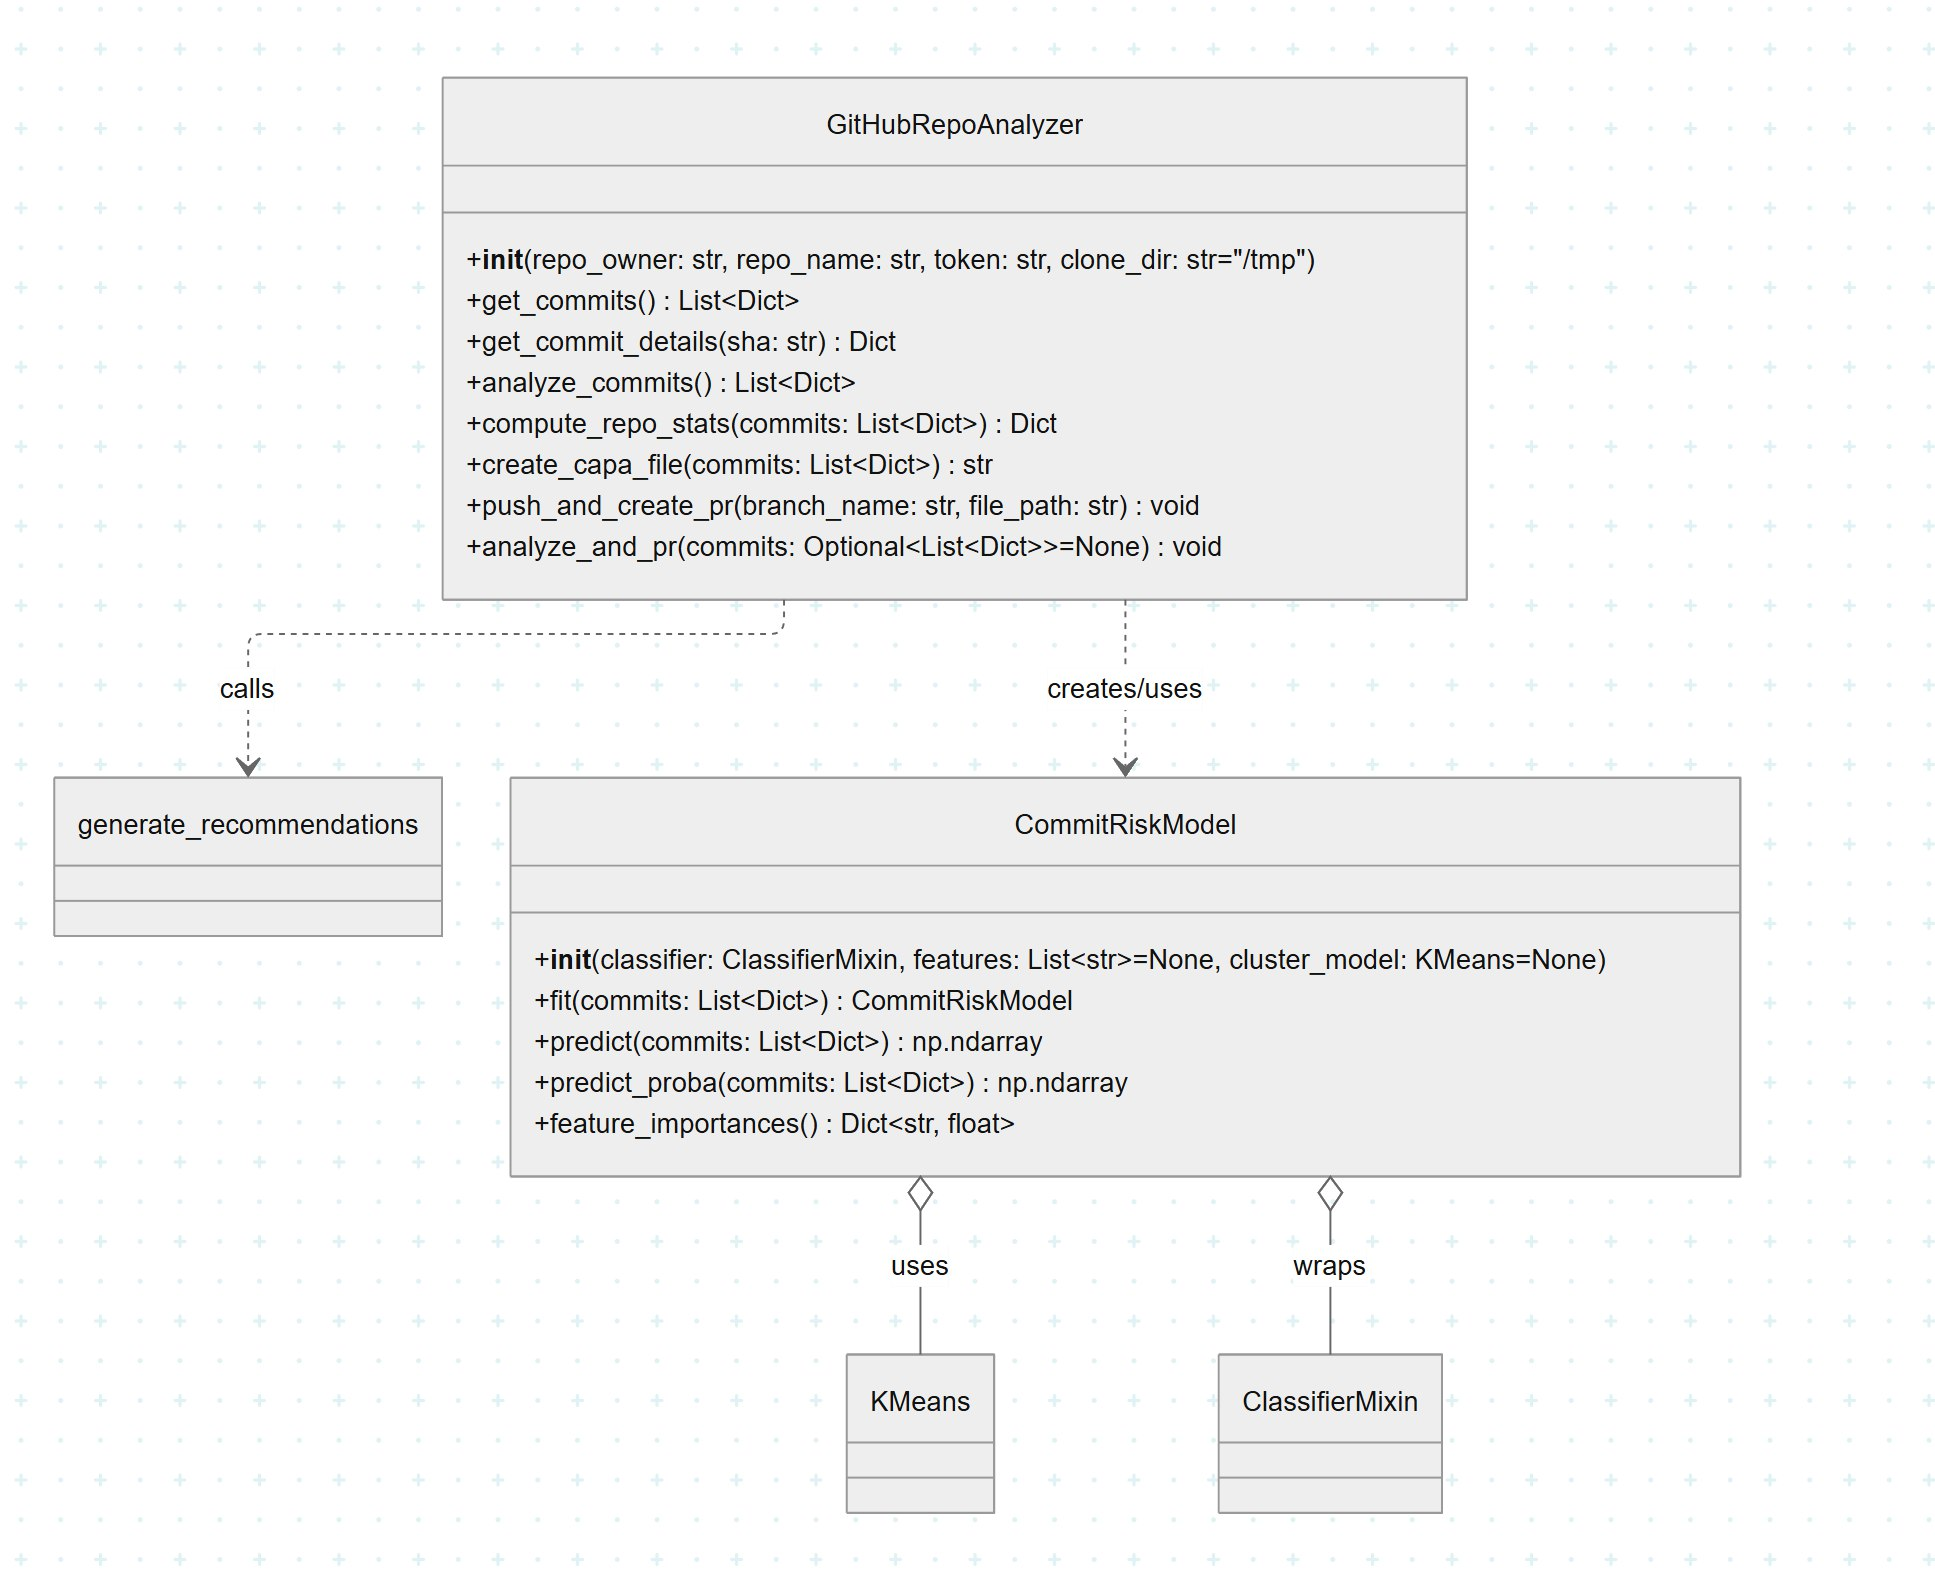
\includegraphics[width=0.85\textwidth]{my_folder/images/classDiagram.jpg}
	\caption{Диаграмма классов системы анализа коммитов и генерации CAPA}
	\label{fig:class-diagram}
\end{figure}

\paragraph{GitHubRepoAnalyzer}
\begin{itemize}
	\item { init(repo\_owner: str,\ repo\_name: str,\ token: str,\ clone\_dir: str="/tmp")}
	\begin{itemize}
		\item Клонирует (или открывает) локальный репозиторий и настраивает REST-клиент GitHub.
	\end{itemize}
	\item { get\_commits(): List<Dict>} — постранично получает историю коммитов через GitHub API.
	\item { get\_commit\_details(sha: str): Dict} — детальные сведения по одному SHA.
	\item { analyze\_commits(): List<Dict>} — для каждого коммита:
	\begin{itemize}
		\item делает \texttt{git checkout},
		\item собирает метрики (добавленные/удалённые строки, файлы, сложность, интервалы),
		\item запускает анализаторы кода (pylint, eslint, checkstyle и пр.),
		\item формирует словарь метрик и возвращает список таких словарей.
	\end{itemize}
	\item { compute\_repo\_stats(commits: List<Dict]): Dict} — агрегирует статистики (среднее, стандартное отклонение, квантили) по всем коммитам.
	\item { create\_capa\_file(commits: List<Dict]): str} — генерирует Markdown-файл с рекомендациями CAPA.
	\item { push\_and\_create\_pr(branch\_name: str,\ file\_path: str): void} — создаёт ветку, пушит изменения и открывает Pull Request.
	\item { analyze\_and\_pr(commits: Optional<List<Dict>>=None): void} — объединяет анализ, модель и генерацию PR в единый конвейер.
\end{itemize}

\paragraph{CommitRiskModel}
\begin{itemize}
	\item { init(classifier: ClassifierMixin,\ features: List<str]=None,\ cluster\_model: KMeans=None)} — сохраняет классификатор и модель кластеризации.
	\item { fit(commits: List<Dict]): CommitRiskModel} — 
	\begin{itemize}
		\item извлекает матрицу признаков из списка коммитов,
		\item генерирует псевдолейблы через \texttt{KMeans},
		\item обучает переданный классификатор.
	\end{itemize}
	\item { predict(commits: List<Dict]): np.ndarray} — возвращает предсказанные метки.
	\item { predict\_proba(commits: List<Dict]): np.ndarray} — возвращает вероятность «аномальности».
	\item { feature\_importances(): Dict<str,float>} — выдаёт важность каждого признака либо напрямую, либо через перестановочный анализ.
\end{itemize}

\paragraph{generate\_recommendations}
\begin{itemize}
	\item Функция, принимающая одну запись коммита, вероятность риска, агрегированные статистики и важности признаков.
	\item Возвращает список текстовых рекомендаций CAPA на основе пороговых значений.
\end{itemize}

\paragraph{Взаимосвязи}
\begin{itemize}
	\item { GitHubRepoAnalyzer} вызывает \texttt{CommitRiskModel} в методе { analyze\_and\_pr} для обучения и предсказания риска.
	\item { GitHubRepoAnalyzer} вызывает функцию { generate\_recommendations} для каждого коммита, передавая ей результаты модели и статистики репозитория.
	\item { CommitRiskModel} “wraps” любой классификатор, реализующий интерфейс \texttt{ClassifierMixin}, и “uses” \texttt{KMeans} для генерации псевдолейблов.
\end{itemize}

Таким образом, на диаграмме отражены ключевые компоненты нашего решения: извлечение и анализ коммитов, классификация риска и генерация рекомендаций CAPA, а также механизм автоматического создания Pull Request в репозитории.

\section{Заключение} \label{ch2:conclusion}

В результате проделанной работы была спроектирована система, способная автоматически извлекать и обрабатывать данные о коммитах из репозиториев GitHub, включая метрики добавленных и удалённых строк, состав файлов и результаты статического анализа. Универсальный класс RepoAnalyzer обеспечит гибкость при подключении новых языковых анализаторов и упрощает расширение системы под дополнительные инструменты качества кода. Компонент классификации на основе машинного обучения и KMeans надёжно выявляет аномальные изменения, комбинируя методы JIT-предсказания дефектов и кластерного анализа. Модуль генерации рекомендаций формирует корректирующие и предупреждающие действия CAPA в виде GitHub-issues или pull request’ов, что облегчает интеграцию с существующими процессами разработки. Интерактивный дашборд, реализованный на Dash и Plotly, демонстрирует ключевые показатели активности репозитория, распределение метрик и отмечает проблемные коммиты в удобном визуальном формате. Масштабируемость решения позволяет обрабатывать сотни коммитов и несколько проектов одновременно, а надёжные механизмы повторных запросов к API и логирования ошибок гарантируют стабильность работы. Расширяемая архитектура упрощает добавление новых языков программирования и сторонних анализаторов через конфигурацию mapping, что минимизирует затраты на сопровождение. Нефункциональные требования по своевременности и интеграции также удовлетворены: анализ может запускаться по расписанию или по вебхукам GitHub, а безопасное хранение токенов обеспечивает защиту учётных данных. Выбранный стек технологий (Python, pandas, scikit-learn, Dash, Plotly) доказал свою эффективность при быстром прототипировании и дальнейшем развитии проекта. Итоговая архитектура демонстрирует баланс между модульностью, производительностью и удобством для конечных пользователей, что делает систему готовой к внедрению и дальнейшему масштабированию.
